\chapter{Data curation}
\label{chap:data}

In the crypto-currency domain, real-time price data is, for most exchanges, freely available. Historical data is oftentimes limited with respect to how far back into past the data is being provided. However, continuously recording real-time data results in a complete historical data set from the time when recording was started and provides the desired data set for this research.
A historical limit order book consisting of states which store every bid and ask posted by traders is commonly referred to as a \textit{complete order book}.
The process to accumulate the data and build the order book is illustrated in a high level pipeline in Figure \ref{fig:data-pipeline} below.
Raw event data is collected from an exchange (Bittrex in our case) and processed in order to form a historical limit order book.
\begin{figure}[H]
    \centering
    \makebox[\linewidth]{
        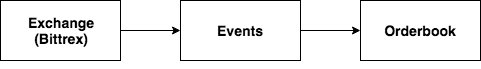
\includegraphics[width=8cm]{data-pipeline.png}
    }
    \caption{Data collection pipeline}
    \label{fig:data-pipeline}
\end{figure}

In this chapter we explain the details of the collection process process and subsequently how a historical order book can be formed thereof, such that it can serve as the historical data source for the match engine.
A sample period of the collected data set is then being investigated in order to find find and visualize properties of the market situation and behaviour of the market participants.
The goal of the investigation is to find hypotheses which state why certain occurrences might be beneficial to consider for the purpose of limit order placement.
Thus, the findings serve as the basis for the feature engineering process which determines the input for the learners as described in Chapter \ref{chap:setup}.

\section{Collection}

There are various ways in order to build a copy of a historical limit order book. However, the only way to rebuild a complete order book is by processing market \textit{events}, that is, every market update for a given ticker (trading pair, in our case USD/BTC).
There are three common types of events, all of which are initiated by a market participant (trader): \textit{order created}, \textit{order cancelled} or \textit{order filled} in case a market order crosses the spread and initiates a trade.

Our exchange of choice for collecting data is Bittrex\footnote{https://bittrex.com/} as the exchange provides a \textit{SignalR}\footnote{https://docs.microsoft.com/en-us/aspnet/signalr/overview/getting-started/introduction-to-signalr} (a library that abstracts \textit{HTTP} and \textit{WebSocket}) interface from which one can extract all status updates (events) from the market.
More specifically, an event in this either a buy- or sell order, or a fill (e.g. trade).
Thus, we subscribe to \texttt{https://socket.bittrex.com/signalr} and filter the data field \texttt{M} for \texttt{updateExchangeState}.
The data type of the message contains the name of the trading pair and a nonce to identify the unique status update in up-counting order.
That is,
\begin{equation}
    StatusUpdate = \{name, nonce, buy_1,...buy_n, sell_1,...sell_n, fill_1,...fill_n\}
\end{equation}
, whereas $buy \in Order_{Limit}$, $sell \in Order_{Limit}$ (see Eq. \ref{eq:order-limit}) and $fill \in Trade$ (see Eq. \ref{eq:trade}).
With that said, the orders hold an additional field $type \in \{0,1,2\}$ which specifies whether it was a \textit{create}, \textit{cancel} or \textit{change} in the order.

As is evident, multiple events can be sent within one status update message. 
We segment the status update into separate events with the same nonce, whereas each event expresses either a limit order of side bid or ask or a filled order resulting in a trade,
\begin{equation}\label{eq:event-update}
    Event = \{name, nonce, type, isTrade, trade, isBid, order\}
\end{equation}
, whereas $isTrade \in \{0,1\}$ and $isBid \in \{0,1\}$ indicating whether the update contains an order or a trade. 
Consequently, $order \in Order_{Limit}$ and $trade \in Trade$.

\section{Order book generation}

The next step is to transform the collected events into an order book structure.
By chronologically iterating over the processed events (Eq. \ref{eq:event-update}), we create a new order book state (Eq. \ref{eq:order-book-state}) for each such event that has a consecutive time stamp.
During this iterative process we follow the rules below, which ensure that the correct order book entries remain in future order book states.
Given the observed event, we act according to the type of the event:
\begin{description}
    \item[Order created:] order book entry is added to the current state.
    \item[Order cancelled:] the amount of shares of the cancelled order is subtracted from the entry in the current state with the corresponding price level.
    \item[Order filled:] the amount of the shares which were traded is subtracted from the entry in the current state with the corresponding price level.
\end{description}
\hfill
\\
As a result, a \textit{list} of order book states is formed which represent a historical order book (Eq. \ref{eq:order-book}).
\textit{We acknowledge that a list representation is by no means the most performing implementation of an order book, but for our purposes it is sufficient.}

\vfill

\section{Understanding the data set}

We take a random period of the recorded data set, representing \textasciitilde10 minutes worth of event data, and try to extract essential information from either raw events or the generated order book.
Our aim is to obtain an understanding of the market situation and how market participants place orders, including some of the properties mentioned in \ref{sec:ob-characteristics}.
We further aim to formulate \textit{hypotheses} which concern why certain properties might be beneficial for the order placement process.
Being aware that the following observations are taken from a random sample of a historical data set, the intent is to make a suggestion which properties might be worth to consider in the feature engineering process.
This is by no means a guarantee that the same observations are true for any order book.

Figure \ref{fig:data-price-movement} below shows the price movement of the sample period, indicating a movement from \$10'100 to \$10'030 and back within 10 minutes.

\begin{figure}[H]
    \centering
    \makebox[\linewidth]{
        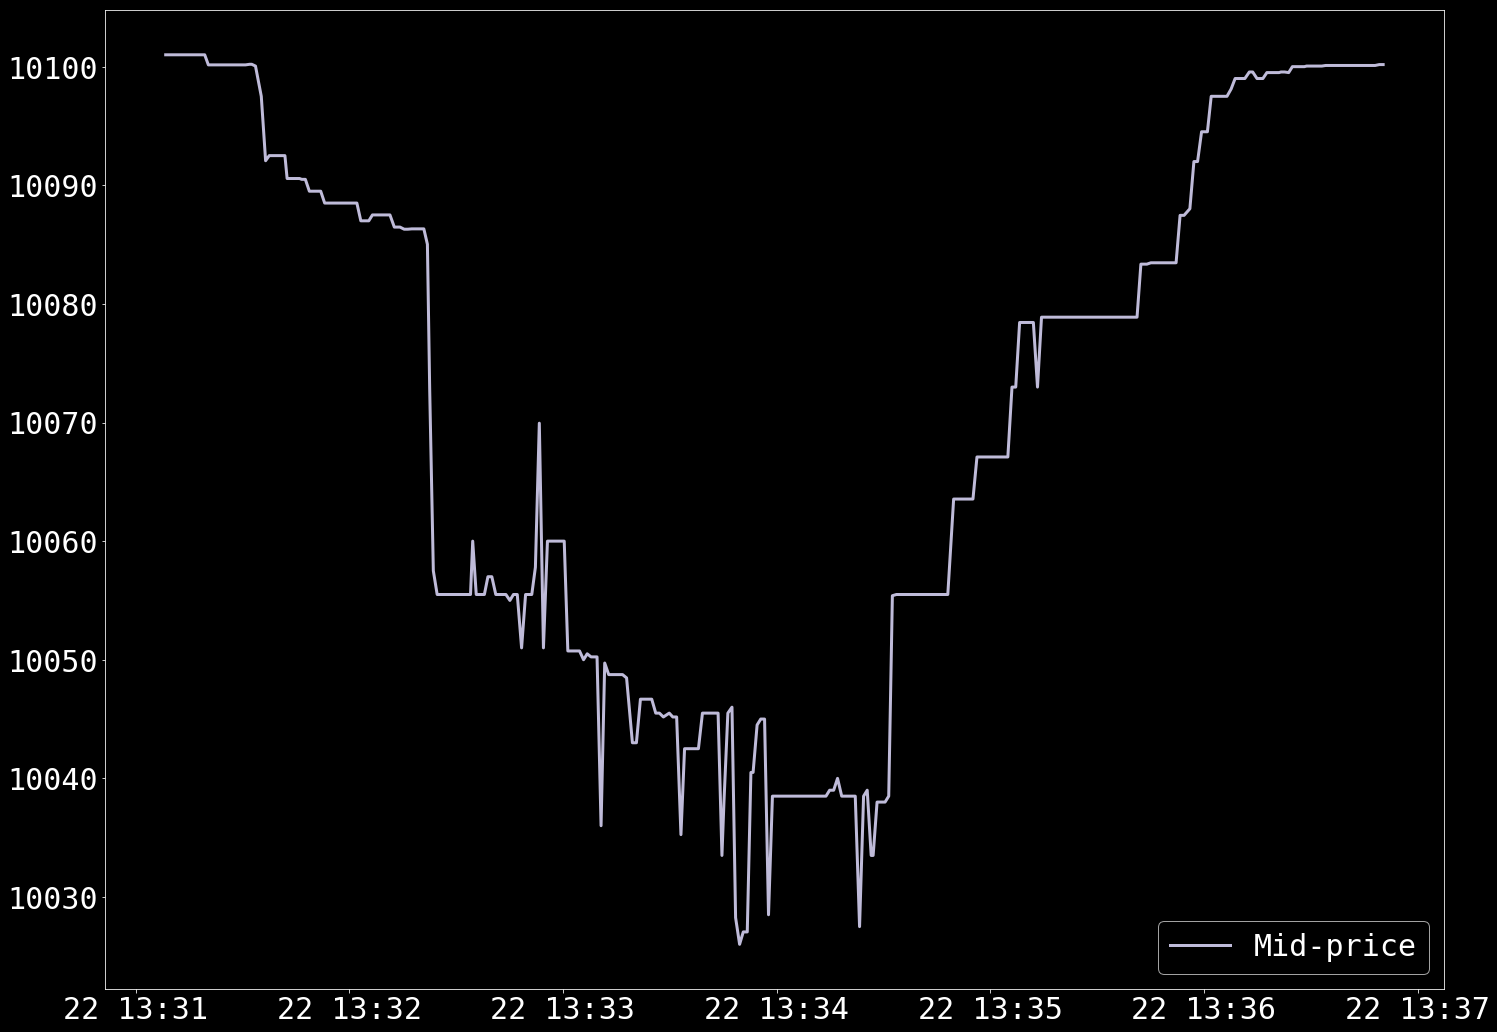
\includegraphics[width=12cm]{ob-price}
    }
    \caption{Price movement of sample data set}
    \label{fig:data-price-movement}
\end{figure}

\subsection{Bid and ask price positioning}

\begin{figure}[H]
    \centering
    \begin{subfigure}[b]{0.45\textwidth}
        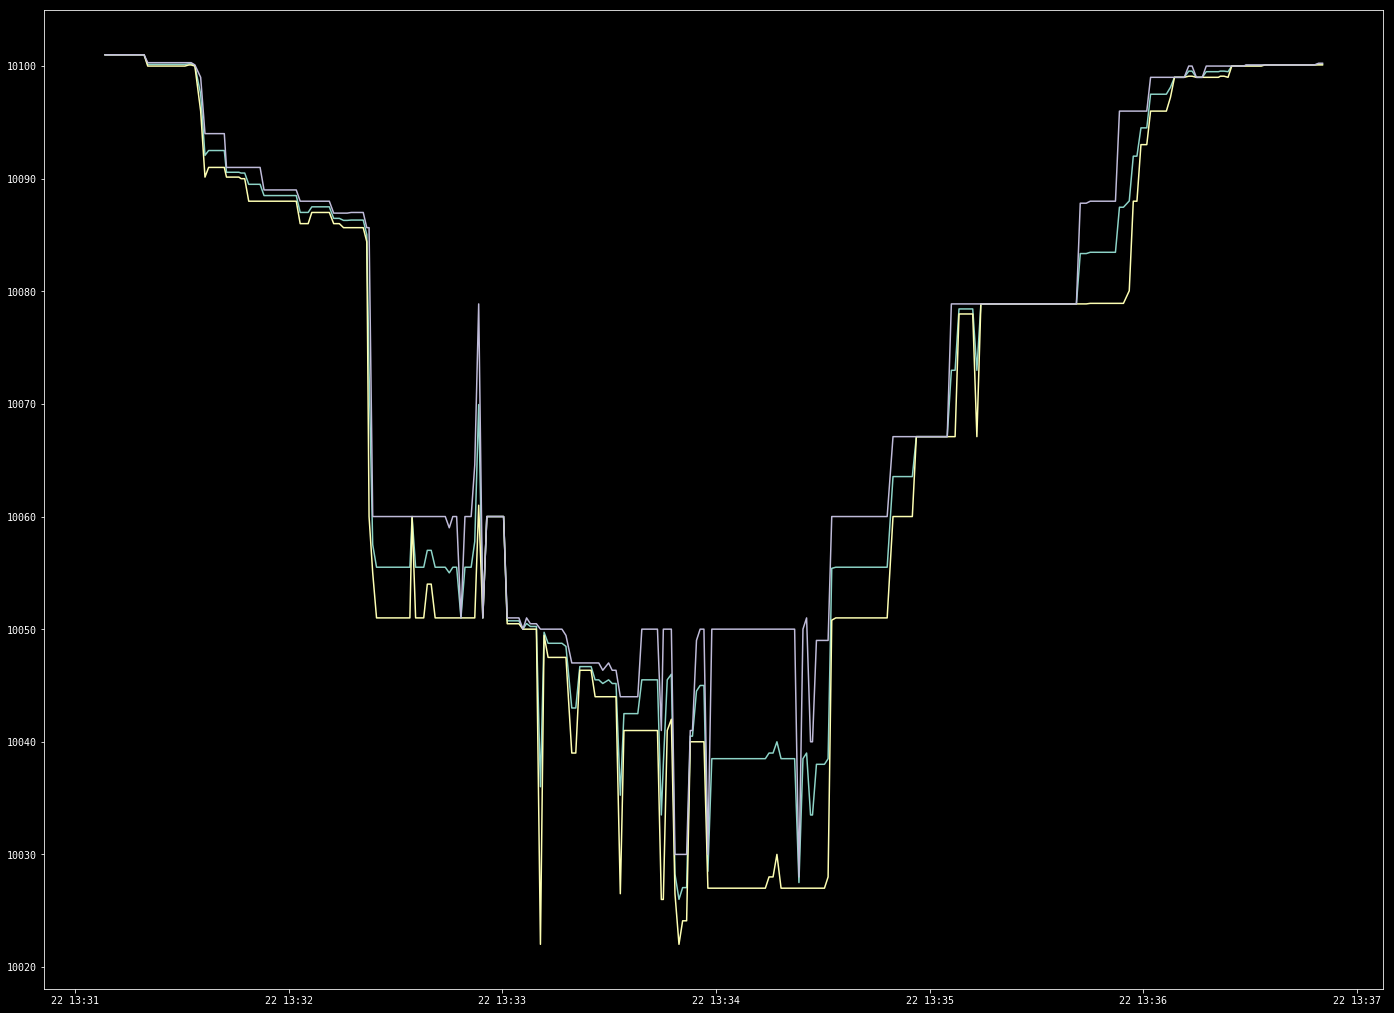
\includegraphics[width=\textwidth]{ob-ba-min}
        \caption{Best bid and best ask}
        \label{fig:ob-ba-min}
    \end{subfigure}
    ~ %add desired spacing between images, e. g. ~, \quad, \qquad, \hfill etc. 
    %(or a blank line to force the subfigure onto a new line)
    \begin{subfigure}[b]{0.45\textwidth}
        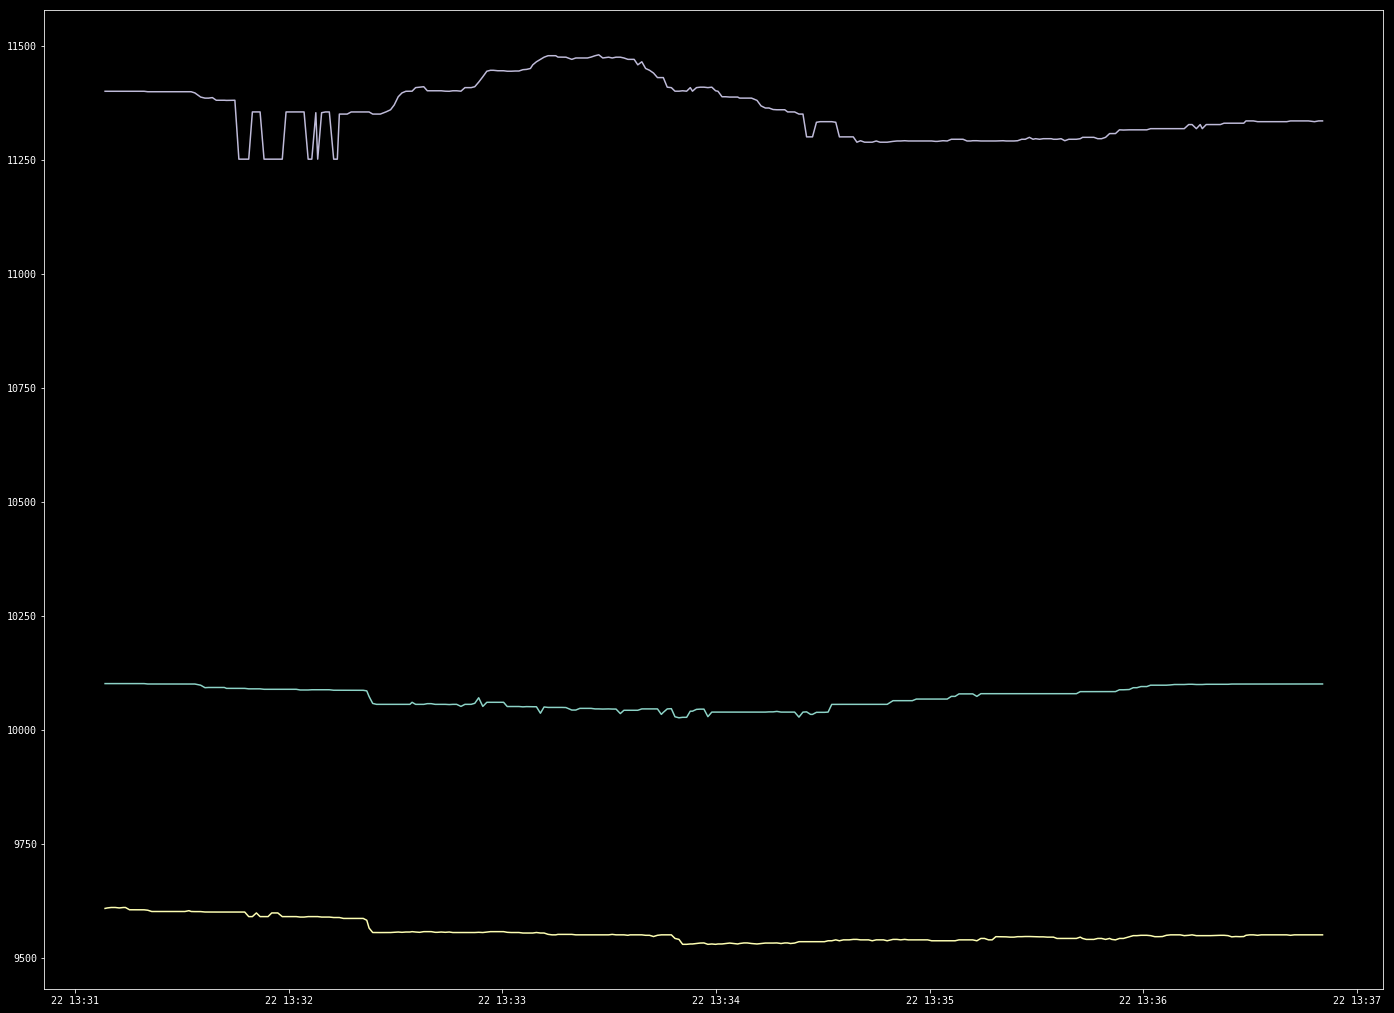
\includegraphics[width=\textwidth]{ob-ba-max}
        \caption{Deepest bid and deepest ask}
        \label{fig:ob-ba-max}
    \end{subfigure}
    \caption{USD/BTC price and bid/ask positions}\label{fig:animals}
\end{figure}

Next we show the same price movement (cyan) but with the best bid (yellow) and ask (violet) (Figure \ref{fig:ob-ba-min}) and the deepest level of bid and ask (Figure \ref{fig:ob-ba-max}).
It is evident that the best bid and ask are close to the price before and after the price dip, meaning the spread is narrow.
During the dip, the spread widens and is at times as large as \$25.
\\
\\
\textit{\textbf{Hypothesis:} participants post offerings close to the spread when the price is stable and start offering with a certain threshold during price fall or rise.}
\\
\\
The orders placed on the deepest level on the buyer and seller side undergo a very interesting change.
Immediately before the the price dip, ask prices start to fluctuate as some participants cancel their listings and possibly others (trader cannot be associated as this is hidden information).
On the contrary, bid prices remain much more stable.
Likewise, during the fall and rise of the price, the ask price starts to increase on the deepest level of the seller side. 
This phenomenon is at first at a first glimpse unexpected as one would expect the sell offers to be lowered as the price falls.
Knowing that the price rises shortly after, it becomes more evident that some sellers ambition was to allure buyers by threatening with higher sell listings.
The ask prices return to the level before the dip as soon as the price starts rising again.
\\
\\
\textit{\textbf{Hypothesis:} sellers allure buyers with higher listings during a price fall.}
\\
\begin{figure}[H]
    \centering
    \begin{subfigure}[b]{0.45\textwidth}
        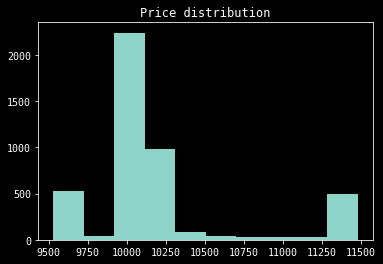
\includegraphics[width=\textwidth]{images/ob-price-bars}
        \caption{Distribution of prices}
        \label{fig:ob-price-dist-unfiltered}
    \end{subfigure}
    \begin{subfigure}[b]{0.45\textwidth}
        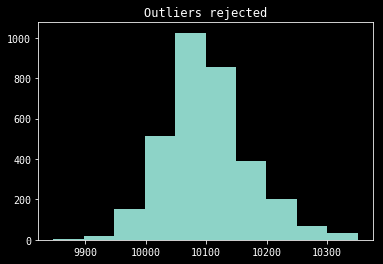
\includegraphics[width=\textwidth]{images/ob-price-bars-rejected}
        \caption{Distribution of prices (filtered)}
        \label{fig:ob-price-dist-filtered}
    \end{subfigure}
    \caption{Price distribution of events}\label{fig:price-distribution}
\end{figure}

Figure \ref{fig:ob-price-dist-unfiltered} shows the distribution of prices of all types of events (create, cancel, trade) within this data set.
As can be seen, most of the events contain prices in the range of the traded price (see Figure \ref{fig:ob-price}) and significantly less below and above this range.
However, the number of events increase with prices on both, the far end of the buyer and seller side, which supports the above stated hypothesis that orders deep in the book might in fact affect the price movement--even though they were not executed within the spectrum of this data set.
We then filter events by rejecting outliers of their price $p$ according to standard deviation $\sigma$, $ |p_i - \overline{p}| < m * \sigma_{p} $, whereas $m=2$.
As a result, Figure \ref{fig:ob-price-dist-filtered} shows the distribution of the prices from the filtered events, that follows a standard distribution.
The mean lays at approximately \$10'100, the price level before and after the dip.
\\
\\
\textit{\textbf{Hypothesis:} in case of a price dip (or raise) density estimation can be applied to find a more stable price level.}

\subsection{Bid and ask volume imbalance}

It was shown that market participants position their offerings at different price levels as the asset price is moving due to trading.
The second variable in posting orders is the volume and we aim to determine whether or not this is a factor which is affected during the previously introduced price movement.

\begin{figure}[H]
    \centering
    \begin{subfigure}[b]{0.45\textwidth}
        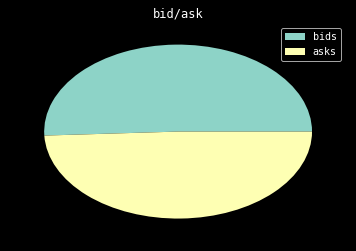
\includegraphics[width=\textwidth]{images/ob-ba-pie-all}
        \caption{All events}
        \label{fig:data-imbalance-events}
    \end{subfigure}
    \begin{subfigure}[b]{0.45\textwidth}
        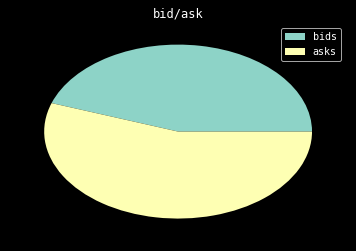
\includegraphics[width=\textwidth]{images/ob-ba-pie-trades}
        \caption{Trades only}
        \label{fig:data-imbalance-trades}
    \end{subfigure}
    \begin{subfigure}[b]{0.45\textwidth}
        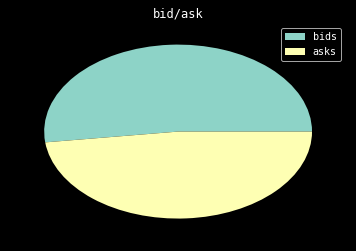
\includegraphics[width=\textwidth]{images/ob-ba-pie-created}
        \caption{Create order only}
        \label{fig:data-imbalance-creates}
    \end{subfigure}
    \begin{subfigure}[b]{0.45\textwidth}
        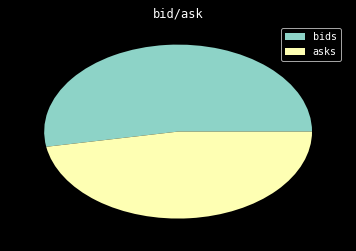
\includegraphics[width=\textwidth]{images/ob-ba-pie-cancelled}
        \caption{Cancel orders only}
        \label{fig:data-imbalance-cancels}
    \end{subfigure}
    \caption{Bid / Ask volume imbalance}\label{fig:data-imbalance}
\end{figure}

Figure \ref{fig:data-imbalance} shows the (im-)balance of the volumes of bid and ask orders segmented as follows.
Figure \ref{fig:data-imbalance-events} shows the ratio of bids and asks of all events, including trades, creations and cancellations. 
Figure \ref{fig:data-imbalance-trades} show the ratio of trades being initiated by either a bid or ask order.
Figure \ref{fig:data-imbalance-creates} demonstrates the ratio of created orders and Figure \ref{fig:data-imbalance-cancels} cancellation orders, again distinguishing between bid and ask.
It is evident that, even though the price moved significantly within the recorded time range, the entirety of the orders is well balanced between trades or orders on the bid side and the ask side.
For trades however, clearly more shares were sold than bought.
It is then evident that the market participants reacted on the sale of the asset by not only creating but also cancelling more buy than sell orders.
We take the last statement as an indication that the market participants may have responded to the price dip by cancelling their current buy orders and posting them deeper in the book (out of fear that the price might fall even further).
Interestingly, even though the price rose after the dip, not as much volume was used on creations and cancellations of orders on the seller side.
\\
\\
\textit{\textbf{Hypothesis:} imbalance of bids and asks of event types indicates future behaviour of participants.}

\subsection{Events investigated over time}

So far, the volume was investigated as a sum of events over time.
In order to understand the behaviour of the participants in greater detail, a \textit{volume map} shall provide better insight into the single events occurred over time.

Figure \ref{fig:data-volmap-crated} shows the volume map of the orders which were created over the time span of the data set.
Hence, the x-axis represents the time stamp and the y-axis is the volume of the placed order.
For visibility reasons and since the majority of the orders have a small volume and fewer have large volume, the y-axis follows a log-scale.
Participants cannot be assigned to such an order, as the trader id is non-public information.
However, as we will see, one can determine some participants according to their behaviour.

\begin{figure}[H]
    \centering
    \makebox[\linewidth]{
        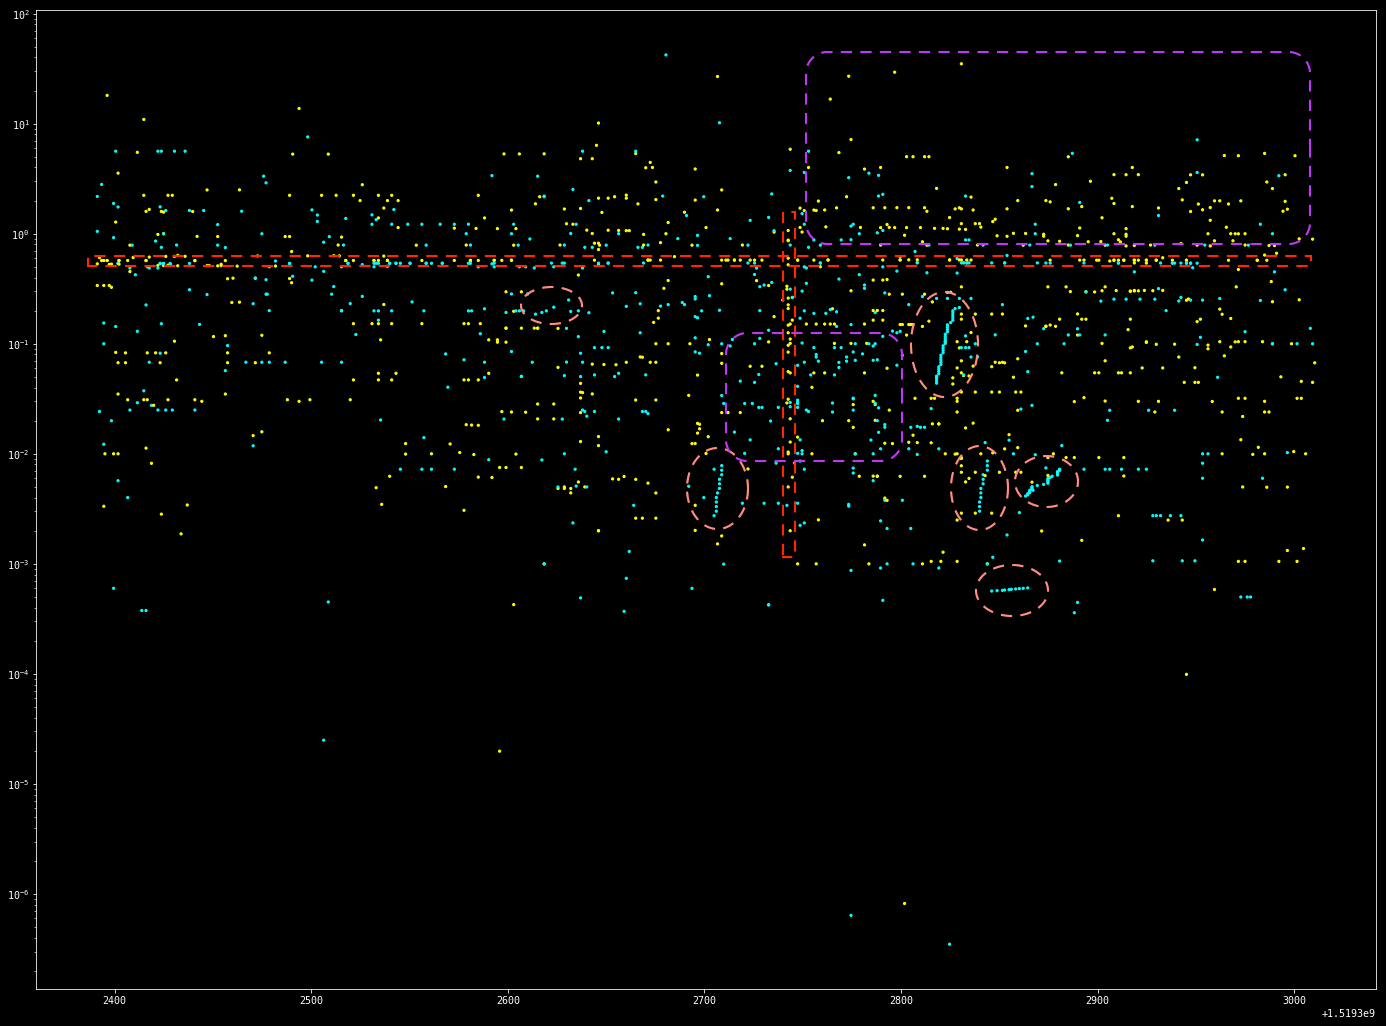
\includegraphics[width=14cm]{images/data-volmap-created}
    }
    \caption{Volume map of created bid (cyan) and ask (yellow) orders.}
    \label{fig:data-volmap-crated}
\end{figure}

What might not be obvious due to the log scaling is the fact that most of the orders were placed with volume between >0 and <0.5 and significantly less with larger volume.
Only a few orders had a volume greater than 10 BTC, meaning that most of the participants either are willing to buy and sell only small quantities or split their orders to minimize the market impact.

From a horizontal perspective, one can detect some orders of both sides, bids and asks, being listed with the same time interval.
Particularly evident is such a behaviour at the volume just below $10^0$.
This is likely one or multiple bots posting orders with the same volume and perhaps at a different price level.
Examples of this behaviour is marked with a red-dashed horizontal box.
A similar behaviour can be seen from a vertical perspective where one or more traders post orders at different price levels, with the same price segmentation.
This is market with a red-dashed vertical box.
Furthermore, a very distinctive pattern is when a trader posts orders within a short period of time but changing volume.
This might be evidence of someone splitting a larger order into small pieces and is marked with an orange-dashed circle.
Some refer to such a behaviour as \textit{buy-wall} (\textit{sell-wall} in case of an ask orders) and surprisingly, this behaviour appeared the most when before and during the price started rising again (compare time stamps from Figure \ref{fig:data-price-movement}).
Last but not least, examples of areas dominated by one particular order side is marked with a purple box.

\begin{figure}[H]
    \centering
    \makebox[\linewidth]{
        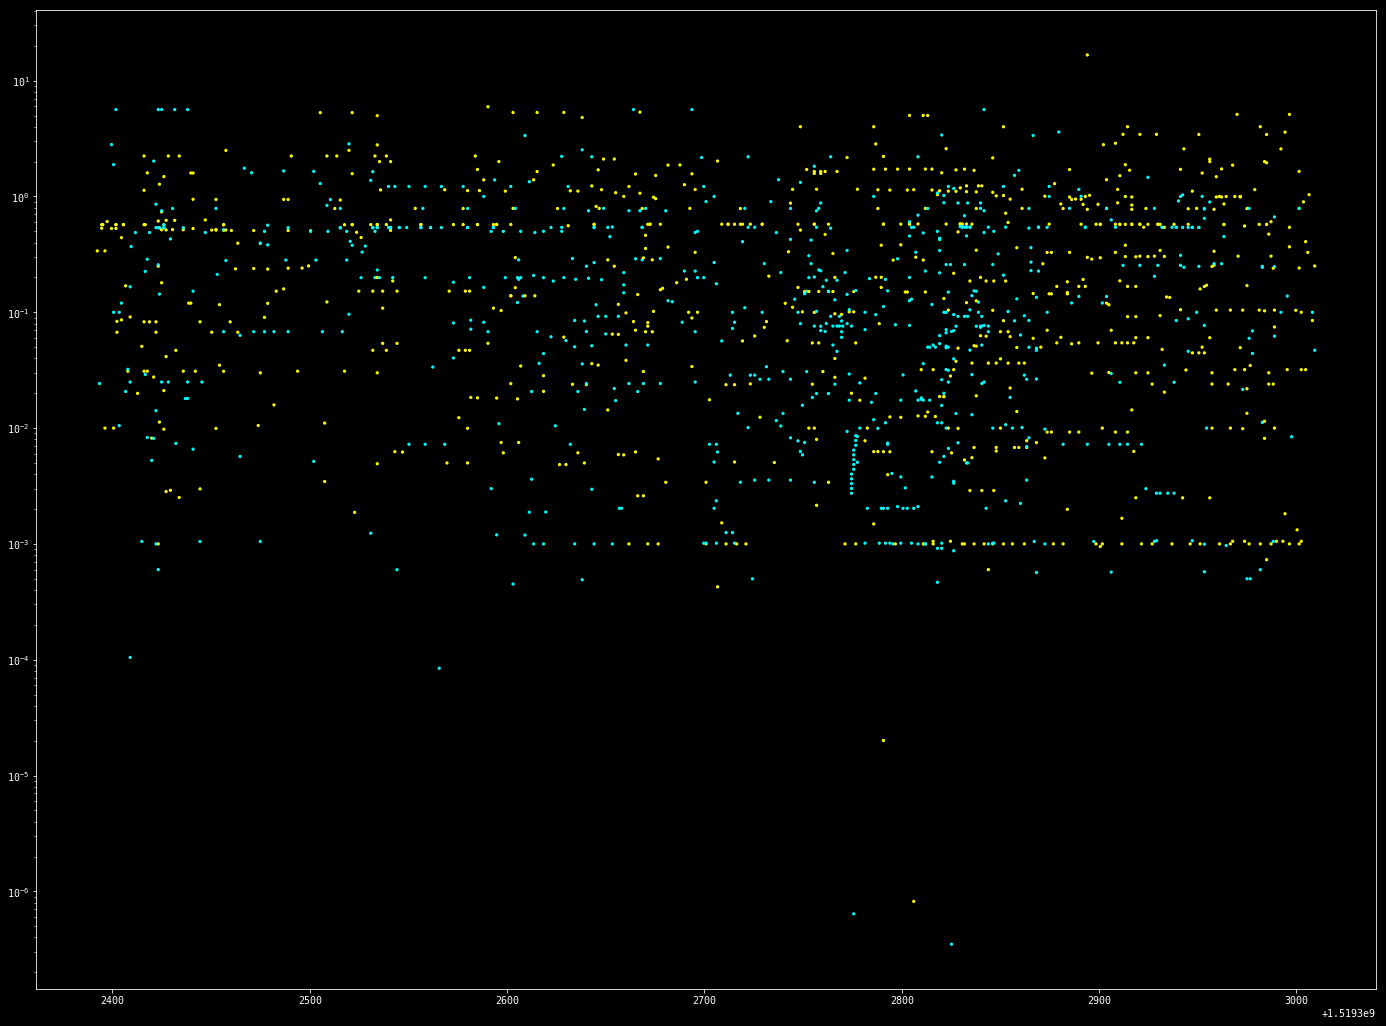
\includegraphics[width=14cm]{images/data-volmap-cancelled}
    }
    \caption{Volume map of cancelled bid (cyan) and ask (yellow) orders.}
    \label{fig:data-volmap-cancelled}
\end{figure}

It is to be expected that at least for some of the orders, which did not result in a trade, a cancellation followed.
Figure \ref{fig:data-volmap-cancelled} therefore shows the cancel orders posted by traders over time.

Continuous cancellations become especially evident at volume levels just below $10^0$ and $10^{-1}$, correlating with the continuous create orders appeared at the same price level above.
Hence, there is likely a trader following some strategy.
A cancellation of one of the created buy-walls is particularly evident at the same time stamp and with equal volumes as previously discovered.
Hence, making it more even more likely that the wall was created and cancelled by a single trader.
\vfill
\pagebreak

\begin{figure}[H]
    \centering
    \makebox[\linewidth]{
        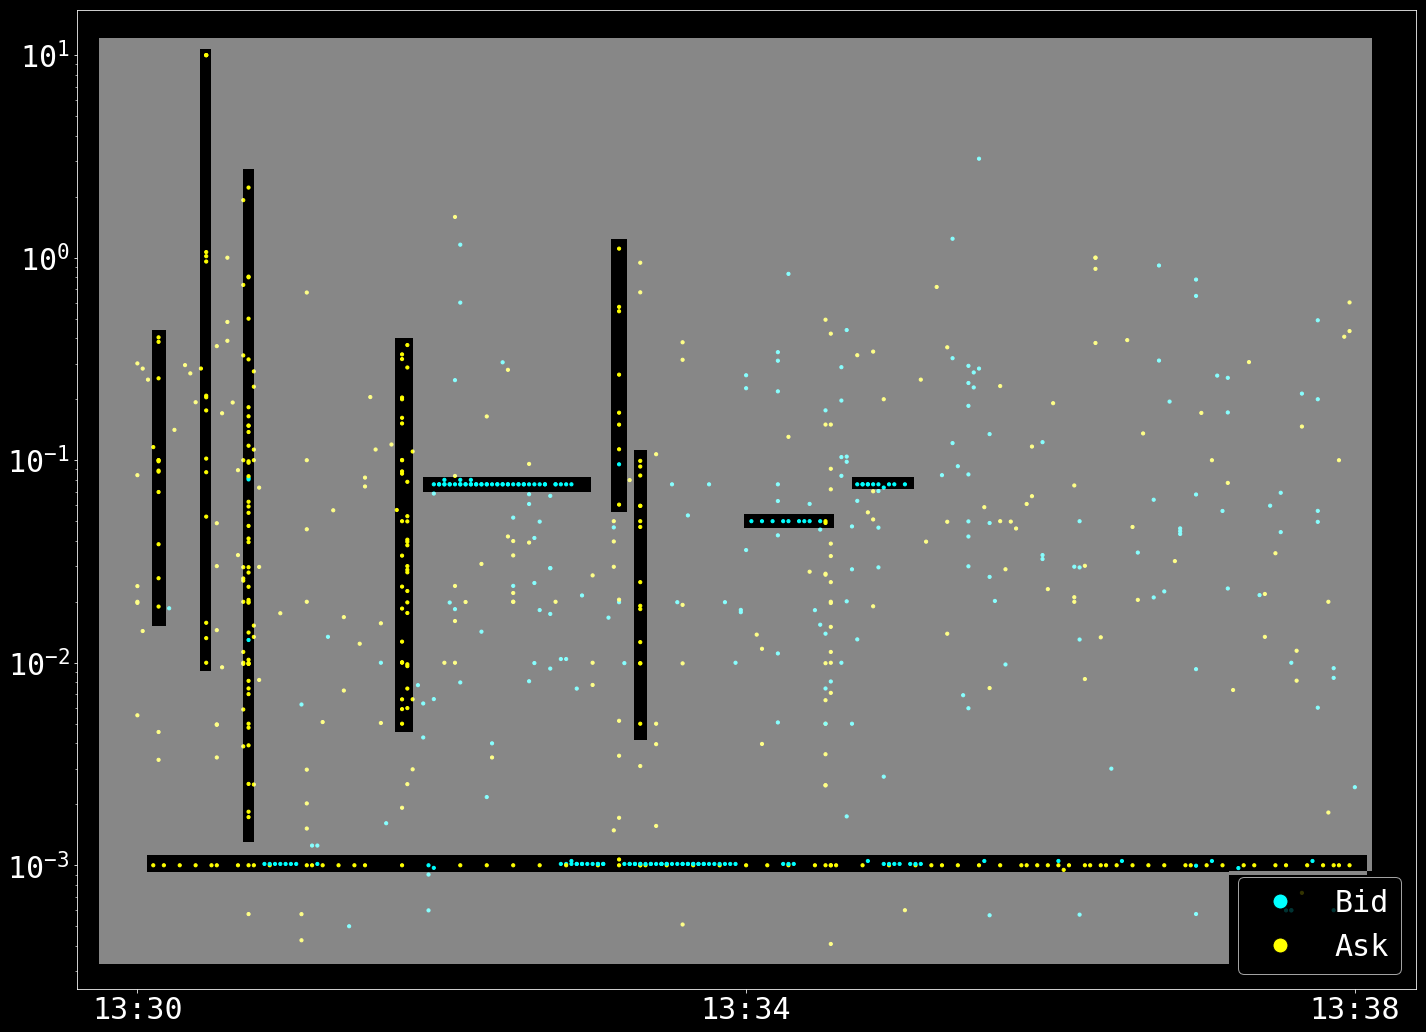
\includegraphics[width=14cm]{images/data-volmap-traded}
    }
    \caption{Volume map of trades initiated by a bid (cyan) or ask (yellow) order crossing the spread.}
    \label{fig:data-volmap-traded}
\end{figure}

So far only posted limit orders or their cancellation where observed.
Not all of those limit orders might have executed and resulted into a trade as there is always a market order required, initiated by one of the two parties involved in a trade.
Figure \ref{fig:data-volmap-traded} therefore illustrates the volume map of the actual trades occurred within this sample time range of the data set.

Immediately evident are the trades transacted with volume $10^{-3}$, with oftentimes identical time interval.
Additionally, an intensive series of consecutive sales occurred at the time when the price dipped.
After the dip, such sales are not present anymore.
Furthermore, intensive and immediate purchases are visible with various volume at some distinctive time stamps before and during the price fall.
We remember that there was one spike towards a higher price during the dip, and the time stamp of which correlates strongly to the purchases visible in this figure.
\\
\\
Various behavioural patterns have been observed by investigating events initiated by market participants over time.
For some, their impact on the market price is immediately obvious, for others it is hard to interpret by hand.
However, an attempt to find correlation between the behaviour of the events and the resulted trades with the application of learning techniques seems promising.
\\
\\
\textit{\textbf{Hypothesis:} patterns arising from posted volume in events can be detected and allow to estimate future short-term trading behaviour which can be exploited in favour of order placement.}

\subsection{Impact of traded price and volume}

The price levels and volume of events over time was investigated for each type in the previous subsections.
Patterns were found and a hypothesis was stated which encourages the various offerings of volume of an order to be an indicator of future behaviour of market participants, which eventually influences the market price and implicitly determines optimal order placement.
The next logical step is to investigate the sum of traded volume at a given point in time (as shown in Figure \ref{fig:data-volmap-traded}) in combination with the price the asset was traded for.

\begin{figure}[H]
    \centering
    \makebox[\linewidth]{
        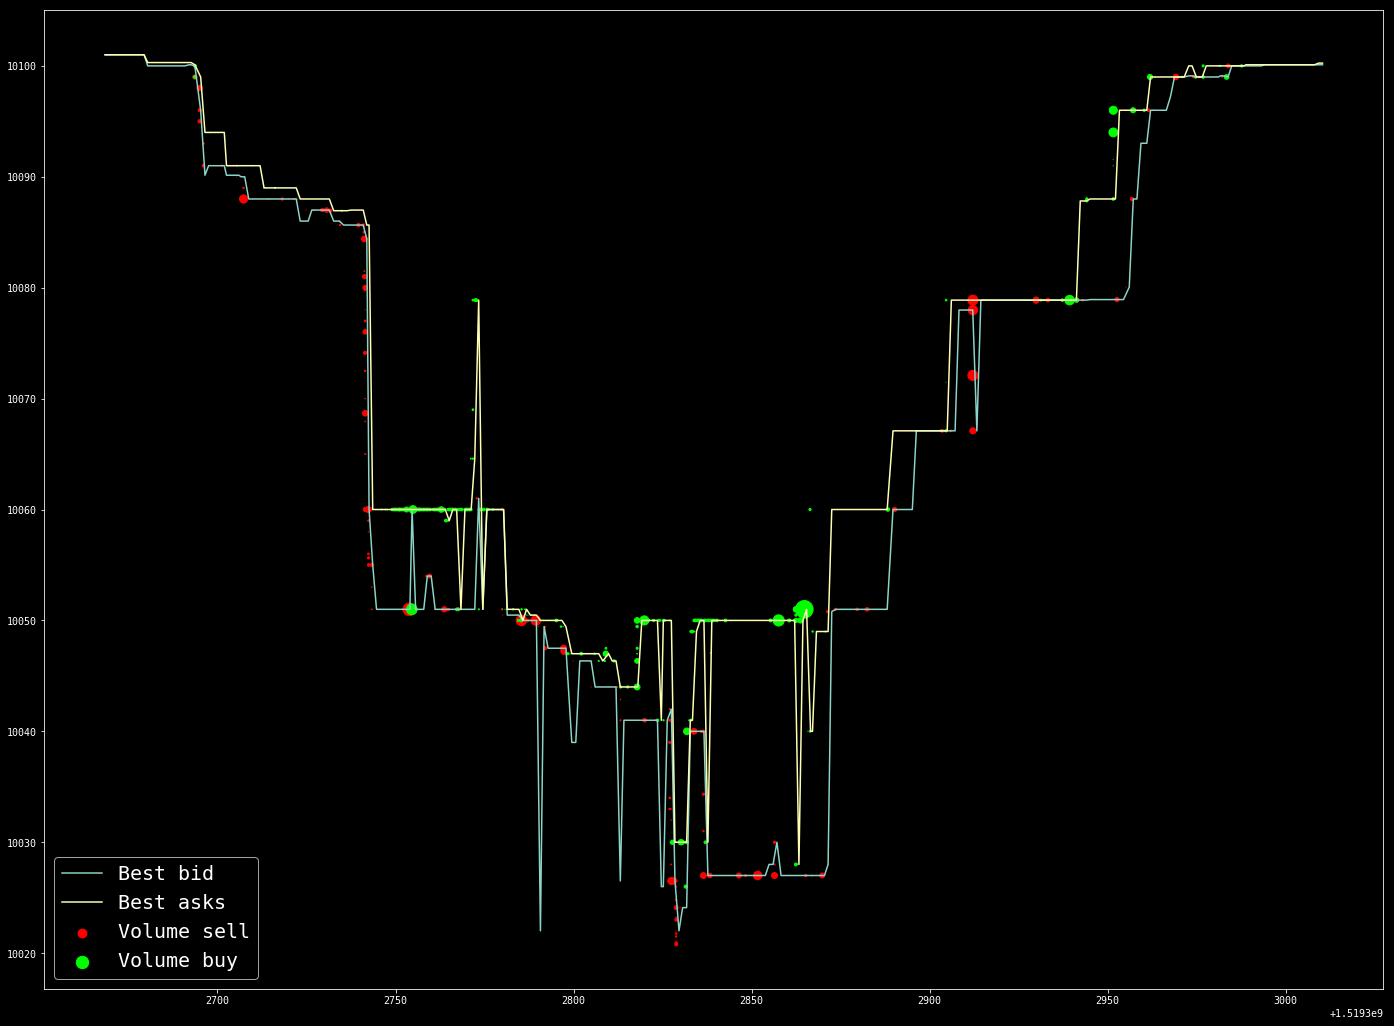
\includegraphics[width=14cm]{data-trade-volume}
    }
    \caption{Relation of trade volume to price movement.}
    \label{fig:data-trade-volume}
\end{figure}

Figure \ref{fig:data-trade-volume} illustrates the volumes of trades on both bid and ask side, which resulted in a buy or sell at a certain price.
The volume of these trades are illustrated as bubbles according to their size (e.g. traded volume) and price.
As is known, a buy appears when one crosses the spread towards the sellers side (ask) and a sell appears when crossing towards the buyer side (bid).
One can clearly see how buys are listed on the best ask price level and sells are listed on the best buy price level.
Before and during the dip sells appear consecutively, followed by a series of buy orders with low volume, which caused the short spike.
Interestingly, a rather large trade caused by a bid appeared shortly before the price started rising again.
Even though sellers confronted the market in the middle of the price rise, participants continued buying shortly after with approximately equal volume.
Concluding this observation it is evident that few trades with small volume caused a certain noise in the overall trend.
Multiple consecutive trades initiated one side or a single large the like, however, led the market price to move for substantially longer period of time.
\\
\\
\textit{\textbf{Hypothesis:} consecutive small or one large trade give an impulse that drives the market price up or down.}

\section{Conclusion}

Event data was collected from a crypto-currency exchange and a limit order book was reconstructed thereof.
The limit order book serves as the historical data set and source for the match engine in order to simulate order placement. 
Subsequently the price chart as the result of the generated order book was shown and an investigation of the underlying event data was proceeded.
Patterns were found which give insight in how market participants positioned their offerings with respect to price and size.
It was shown that the price movement was likely due to (1) an imbalance in bid and ask orders; (2) a distinctive way of posting or cancelling orders; and (3) consecutive or impulsive trades.
Hence, the findings in this chapter serve as the basis for the feature engineering process. 